\begin{frame}
  \begin{floatingfigure}[rh]{0.2\textwidth}
    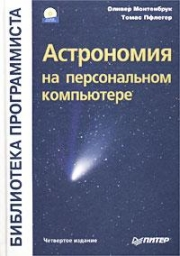
\includegraphics[width=0.2\textwidth]{astro.jpg}
  \end{floatingfigure}
  
  \begin{itemize}
  \item Тег canvas (HTML5), раз в 15 секунд.
  \item starjs для расчётов.  О.~Монтенбрук, Т.~Пфлегер. "<Астрономия
    на персональном компьютере">.
  %\item Стереографическая проекция.
  \end{itemize}
\end{frame}
%%% Local Variables: 
%%% mode: latex
%%% TeX-master: "presentation"
%%% End: 
